\documentclass[conference]{IEEEtran}
\IEEEoverridecommandlockouts
\usepackage{cite}
\usepackage{amsmath,amssymb,amsfonts}
\usepackage{algorithmic}
\usepackage{graphicx}
\usepackage{textcomp}
\usepackage{xcolor}
\usepackage{url}
\usepackage{subcaption}
\def\BibTeX{{\rm B\kern-.05em{\sc i\kern-.025em b}\kern-.08em
    T\kern-.1667em\lower.7ex\hbox{E}\kern-.125emX}}
\begin{document}

\title{Physical Presence-Based Authentication and Authorization for Cyber-Physical Systems and IoT using LiFi}

\author{\IEEEauthorblockN{1\textsuperscript{st} Jose Felix}
\IEEEauthorblockA{\textit{KIM Labs} \\
\textit{Arizona State University}\\
Tempe, Arizona \\
jmfelix4@asu.edu}
\and
\IEEEauthorblockN{2\textsuperscript{nd} Dongha Kim}
\IEEEauthorblockA{\textit{KIM Labs} \\
\textit{Arizona State University}\\
Tempe, Arizona \\
dongha@asu.edu}
\and
\IEEEauthorblockN{3\textsuperscript{rd} Hokeun Kim}
\IEEEauthorblockA{\textit{KIM Labs} \\
\textit{Arizona State University}\\
Tempe, Arizona \\
hokeun@asu.edu}
\and
\IEEEauthorblockN{4\textsuperscript{th} Michel Kinsy}
\IEEEauthorblockA{\textit{STAM Center, School of Computing and Augmented Intelligence} \\
\textit{Arizona State University}\\
Tempe, Arizona \\
mkinsy@asu.edu}
\and
\IEEEauthorblockN{5\textsuperscript{th} Gail-Joon Ahn}
\IEEEauthorblockA{\textit{School of Computing and Augmented Intelligence} \\
\textit{Arizona State University}\\
Tempe, Arizona \\
gahn@asu.edu}
}

\maketitle

\begin{abstract}
LiFi (Light Fidelity) is an emerging optical communication method that transmits data using visible and invisible light modulated imperceptibly to the human eye. While secure access control in IoT environments increasingly demands verification of physical presence, existing wireless approaches — including RF-based protocols such as WiFi and Bluetooth — cannot reliably enforce physical boundaries, as signals propagate beyond intended spaces and remain vulnerable to relay and replay attacks. No widely adopted solution currently exists that binds authorization directly to continuous physical presence in real time. Using a Raspberry Pi-based embedded platform equipped with a photodiode receiver, this system enforces continuous physical alignment between sender and receiver, binding the receiving device to a specific physical location. Session key provisioning and per-device dynamic key rotation are managed through the SST (Secure Swarm Toolkit) IoTAuth framework, delivered exclusively over the LiFi optical channel. The system is validated through a physical prototype achieving authenticated encrypted optical communication at 1 Mbps, with the receiver implemented on a custom PCB designed for direct integration with a mobile robotic platform — demonstrating a practical, real-world application of LiFi in high-security environments, where alternative wireless approaches either cannot enforce physical boundaries or require costly environmental modification to do so. This work establishes that authorization can be bound to continuous physical optical presence, such that access is automatically revoked upon signal interruption, making light itself a verifiable and unforgeable proof of presence.
\end{abstract}

\begin{IEEEkeywords}
LiFi, visible light communication, physical presence, authentication, authorization, IoT security, AES-GCM, cyber-physical systems, optical wireless
\end{IEEEkeywords}

\section{Introduction}

The rapid proliferation of cyber-physical systems (CPS) — in which computational processes are tightly coupled with physical environments and real-world actuation — has fundamentally expanded the attack surface of modern infrastructure. From autonomous robotics and industrial control systems to smart access control and unmanned aerial vehicles, CPS deployments demand security guarantees that extend beyond traditional network boundaries into the physical world. Modern IoT infrastructure, which forms the sensing and communication backbone of many CPS environments, relies overwhelmingly on radio frequency (RF) wireless protocols — including WiFi (IEEE 802.11), Bluetooth, and Zigbee — to connect and authenticate devices. While these technologies offer broad coverage and ease of deployment, their fundamental physical property of propagating through walls, floors, and physical barriers creates an inherent security limitation: an attacker need not be physically present to intercept, relay, or replay an authorization credential. This property makes RF-based systems structurally incapable of enforcing physical presence as a security boundary without deliberate and costly modification of the physical environment — such as RF shielding, Faraday enclosures, or signal attenuation infrastructure — placing the security burden on architecture rather than protocol design.

Light-emitting diodes (LEDs) have undergone a quiet but transformative proliferation over the past two decades, becoming the dominant illumination technology across virtually every indoor environment. Hospitals, schools, warehouses, office complexes, and government facilities have nearly universally transitioned to LED infrastructure — driven primarily by energy efficiency mandates and cost reduction — yet the full communicative potential of this installed base remains almost entirely untapped. A standard LED can be modulated at frequencies imperceptible to the human eye, switching on and off millions of times per second while maintaining its apparent steady illumination. This property, the foundation of Light Fidelity (LiFi) communication, transforms an already-deployed, already-powered, and already-trusted physical infrastructure into a parallel communication and authorization channel — one that requires no additional radio spectrum allocation in an era where RF spectrum congestion is an escalating constraint on wireless capacity.

Every classroom equipped with LED overhead lighting is, in principle, a facility capable of spatially scoped, eavesdrop-resistant communication. Every hospital ward, where RF emissions are already constrained or prohibited near sensitive medical equipment, possesses a ready-built optical network that could simultaneously illuminate and authorize. Every secure government operations center, every industrial floor where RF interference poses operational risk, every access-controlled server room — all represent environments where the convergence of illumination infrastructure and communication security is not merely convenient but architecturally natural. Unlike RF-based approaches, which require deliberate countermeasures to confine their propagation, optical communication is confined by construction: light does not pass through opaque walls, does not propagate around corners without deliberate redirection, and does not travel from one room to the next without physical intervention.

This work exploits that property not solely as a communication channel but as an active security primitive. Rather than treating LiFi as a higher-bandwidth wireless alternative, we reframe the optical signal itself as a verifiable proof of physical presence — one that is continuously asserted, continuously verified, and automatically revoked the moment the optical path between sender and receiver is broken. This shifts the security model from a question of credential possession to a question of physical geometry: authorization is granted not because a device holds a valid key, but because it is, at this moment, in this exact location, receiving light from this specific source.

\section{Related Work}

\subsection{LiFi as a Communication Technology}
The term LiFi was first introduced by Harald Haas in his 2011 TEDGlobal talk~\cite{haas2011}, where he demonstrated that a standard LED bulb, modulated at speeds imperceptible to the human eye, could transmit data at rates exceeding conventional RF wireless technologies. Since then, the IEEE 802.11bb standard~\cite{ieee80211bb}, ratified in June 2023, specifies bidirectional optical PHY layers that achieve throughputs between 10\,Mb/s and 9.6\,Gb/s, operating in the 800\,nm to 1000\,nm near-infrared band — establishing LiFi as a formally recognized wireless standard with measurable and interoperable performance guarantees. Under experimental conditions, researchers have demonstrated peak data rates of 224\,Gb/s — exceeding the fastest commercial Wi-Fi implementations by two orders of magnitude.

\subsection{RF-Based State of the Art}

Wi-Fi RSSI fingerprinting represents the most widely deployed RF-based approach to indoor presence estimation, operating by matching a device's received signal strength profile against a pre-built spatial database. However, the approach is fundamentally probabilistic — RSSI values fluctuate with human movement, temperature variation, multipath propagation, and environmental change, producing positioning errors that routinely reach several meters under real-world conditions. More critically, WiFi signals are designed for broad coverage and penetrate most walls, meaning the authorization boundary does not coincide with the physical boundary of a space. Research has demonstrated that a passive adversary equipped with nothing more than a commodity smartphone can monitor and manipulate RSSI readings from outside a building — without ever accessing the network, the devices, or the space itself. An attacker who can estimate the distance between transmitter and receiver can simply amplify transmission power to spoof a matching RSS value, defeating presence-based authentication from outside the intended boundary. The result is a system where the authorization perimeter exists in software policy, not in physical law — and is therefore subject to manipulation by any sufficiently motivated adversary with commodity hardware.

\subsection{Physical Layer Security}

Physical layer security as a formal discipline originates with Wyner's landmark 1975 wiretap channel model, which demonstrated that secure communication is achievable without a shared secret key when the legitimate receiver's channel is of higher quality than the eavesdropper's~\cite{wyner1975}. This theoretical foundation motivated decades of subsequent work — channel reciprocity key generation, cooperative jamming, and beamforming — all attempting to engineer a favorable channel advantage for legitimate parties over adversaries. However, these approaches share a common ceiling: secrecy capacity in RF environments is highly sensitive to environmental dynamics, multipath propagation, and physical changes, making deterministic security guarantees structurally difficult to achieve regardless of protocol sophistication.

To address relay attacks specifically — where an adversary forwards authentication exchanges to falsely assert physical proximity — Brands and Chaum introduced distance-bounding protocols in 1993, using round-trip signal timing to compute an upper bound on the prover-to-verifier distance~\cite{brands1993}. While foundational, these protocols remain vulnerable to mafia fraud and terrorist fraud, and critically, they bound distance without enforcing location — they answer how far but not where. A system confined by the physics of light answers both simultaneously, with no timing infrastructure, no cryptographic round-trip overhead, and no residual relay vulnerability.

\subsection{VLC and LiFi Security}

The security landscape of visible light communication has been surveyed from multiple perspectives. Blinowski~\cite{blinowski2019} provided the first comprehensive review of VLC security, systematically cataloging threats including eavesdropping, jamming, and node compromise, and organizing countermeasures into physical layer security (PLS), key generation, steganography, and conventional cryptographic approaches. Arfaoui et al.~\cite{arfaoui2020} extended this with a unified treatment of PLS for VLC from both information-theoretic and signal processing viewpoints, covering channel models, input distributions, precoding strategies, and secrecy capacity analysis. Both surveys conclude that despite the spatial confinement of light, VLC systems remain vulnerable in open areas, multi-user scenarios, and rooms with reflective surfaces or windows --- contradicting the common assumption that optical links are inherently eavesdropping-proof.

\subsubsection{Information-Theoretic Physical Layer Security}
The dominant thread in VLC security research derives from Wyner's wiretap channel model, adapted to the optical intensity channel. Researchers have characterized the secrecy capacity of VLC links under various constraints --- non-negative signaling, peak and average optical power limits, and dimmable illumination requirements --- that distinguish VLC from conventional RF analysis. Beamforming techniques using multi-element LED arrays have been proposed to steer optical power toward legitimate receivers while creating nulls at eavesdropper locations~\cite{arfaoui2020}. Protected zones --- eavesdropper-free regions around the receiver --- have been analyzed to quantify the secrecy capacity improvement when physical access control limits how close an adversary can approach~\cite{cho2018}. More recently, intelligent reflecting surfaces (IRS) have been introduced to VLC security, enabling dynamic control of the optical propagation environment to simultaneously enhance legitimate signal quality and degrade eavesdropper reception~\cite{irs_vlc2024}.

These approaches share a common limitation: they provide probabilistic secrecy guarantees that depend on channel state information, eavesdropper location models, and assumptions about the spatial distribution of adversaries. They do not provide deterministic, real-time authorization decisions. A legitimate receiver that moves out of the secure zone or loses line-of-sight continues to be ``authorized'' in any access control sense --- the physical layer security only ensures that an eavesdropper in a disadvantaged position cannot decode the signal. No mechanism exists to revoke the receiver's authorization based on its ongoing physical relationship to the transmitter.

\subsubsection{Physical Layer Key Generation}

A second active research direction exploits the reciprocity and spatial variability of VLC channels to generate shared secret keys between communicating parties without prior key distribution. Al-Moliki et al.~\cite{almoliki2017} proposed a key generation scheme for inter-vehicular VLC that extracts randomness from channel measurements, achieving key generation rates that vary with the relative positions and velocities of the vehicles. More recently, key generation protocols for indoor VLC using OFDM subcarrier measurements have been proposed, leveraging the spatial dependence of the optical channel to ensure that an eavesdropper at a different location derives a different key~\cite{keygen_ofdm2017}. Quantum key distribution over VLC channels has also been explored as an extension to post-quantum security, though practical implementations remain limited to laboratory demonstrations~\cite{qkd_vlc2025}.

Physical layer key generation addresses the key establishment problem but does not address continuous authorization. Once a key is generated and shared, the VLC channel's role in the security protocol ends --- the key persists independently of whether the optical link is maintained. An adversary who obtains the key through any means (side channel, device compromise, relay during the key generation phase) retains it regardless of physical presence.

\subsubsection{VLC-Assisted Device Initialization}

Saxena et al.~\cite{lisa2019} proposed LISA, a multichannel protocol that uses VLC from smartphone screens to securely initialize resource-constrained IoT devices. The visible light channel serves as an out-of-band (OoB) channel for bootstrapping cryptographic credentials, exploiting the assumption that an attacker cannot simultaneously observe the screen and the device without being physically present during the initialization ceremony. This work represents the closest conceptual antecedent to our approach in that it leverages the spatial confinement of light for a security purpose beyond simple data confidentiality. However, LISA uses VLC as a one-time initialization channel --- a brief optical ceremony that establishes long-lived credentials. Once initialization is complete, the optical channel plays no further security role, and the device's authorization does not depend on continued optical reception.

\subsubsection{Encrypted VLC Implementations}

Several hardware implementations of secure VLC have been demonstrated. Kim et al.~\cite{kim2020} implemented an asymmetric RSA-encrypted VLC link using embedded microcontrollers and OOK modulation, achieving secure transmission over short distances with an LED array and photodiode receiver. Liao et al.~\cite{liao2021} demonstrated a chaos-synchronized VLC system using Arduino Due microcontrollers, encrypting audio signals with a R\"{o}ssler chaotic system before optical transmission. These implementations validate that encryption is feasible on resource-constrained VLC hardware, but treat the optical link as a transparent data pipe --- the encryption provides confidentiality in transit, but the physical properties of the optical channel are not themselves used as a security mechanism.

\subsubsection{Commercial LiFi Security}

Industry deployments have begun to address VLC security at the product level. Signify's Trulifi platform offers FIPS 140-3 validated encryption for LiFi connections, marketing the physical confinement of light as an inherent security advantage over RF~\cite{signify2024}. Oledcomm similarly positions LiFi as intrinsically more secure than WiFi due to the non-penetration of light through walls~\cite{oledcomm2024}. The LiFi Lab consortium has proposed a LiFi-based access control system combining optical data transmission with biometric authentication~\cite{lifilab2024}. While these commercial systems leverage the spatial properties of light to reduce the attack surface, they implement conventional authentication models --- a device authenticates once and retains access until explicitly revoked by an administrative action or credential expiry. The continuous physical presence of the device within the optical coverage area is not monitored or enforced as a condition of ongoing authorization.

\subsubsection{The Gap: Continuous Optical Presence as an Authorization Primitive}

Across the existing literature, VLC security research falls into four categories: (1)~information-theoretic analysis of secrecy capacity, which provides statistical guarantees about eavesdropper disadvantage but not real-time authorization; (2)~physical layer key generation, which bootstraps shared secrets from channel measurements but decouples the key from ongoing optical presence; (3)~encrypted VLC implementations, which protect data in transit but do not exploit the physical channel for access control; and (4)~commercial LiFi products, which market spatial confinement as a feature but implement one-time authentication models.

No existing work binds authorization to continuous, time-bounded optical reception with automatic revocation upon signal loss. The concept of presence-based authorization --- in which a device is authorized not because it possesses a credential, but because it is, at this moment, receiving authenticated optical transmissions from a specific source --- has not been formalized, implemented, or evaluated in the VLC security literature. This is the gap that the present work addresses.

\section{System Architecture}

The system comprises three principal subsystems: (1)~an optical transmitter built on the RP2040 microcontroller (Raspberry Pi Pico), (2)~an optical receiver built on the RP2350 microcontroller (Raspberry Pi Pico~2) with a custom analog front-end, and (3)~a key provisioning service based on the SST (Secure Swarm Toolkit) IoTAuth framework running on a Linux host.

\subsection{Optical Transmitter}

The transmitter is responsible for accepting plaintext input, encrypting it under AES-128-GCM, framing the ciphertext with a synchronization preamble and integrity check, and modulating the result onto four LED channels simultaneously via hardware state machines.

\subsubsection{PIO-Based Parallel Transmission}

The RP2040's Programmable I/O (PIO) subsystem is used to implement a custom 8N1 UART transmitter that drives four GPIO pins (GP6--GP9) in lockstep, each connected to a separate LED channel (white, green, blue, red) through a TC4420COA low-side MOSFET gate driver (Microchip, 4.5\,A peak output, 8-SOIC) driving a Vishay SIR800DP-T1-GE3 N-channel MOSFET (40\,V, 80\,A, PPAK) per channel. The LED array operates directly from the 12\,V input rail switched by the MOSFET low-side stage. The PIO state machine executes at exactly 8 cycles per bit, yielding deterministic timing with zero CPU involvement during transmission. At a system clock of 125\,MHz and a target baud rate of 1\,Mbps, the clock divider is set to $125{,}000{,}000 / (1{,}000{,}000 \times 8) = 15.625$.

The use of four parallel LED channels transmitting identical data provides optical redundancy: the receiver need only detect any one channel, and future work can exploit the independent channels for spatial multiplexing or per-channel encoding.

\subsubsection{Sender Power Architecture}

The sender PCB accepts a 12\,V DC input through a Würth Elektronik screw-terminal connector. A Texas Instruments PTN78000WAH wide-input DC-DC module (input range 4.5--14\,V, output set to 5\,V by a 732\,$\Omega$ programming resistor) provides a regulated 5\,V supply to the RP2040 VSYS pin, isolating the microcontroller logic from the high-current switching of the LED stage. Input protection is provided by a Littelfuse SMAJ30A 30\,V TVS clamp diode and a 3.5\,A 1206 chip fuse. Decoupling capacitors (47\,$\mu$F and 220\,$\mu$F electrolytic, 0.1\,$\mu$F ceramic per gate driver) are placed at each switching node to suppress transients.

\subsubsection{Cryptographic Pipeline}

Before transmission, each plaintext message passes through the following pipeline:

\begin{enumerate}
\item \textbf{Encryption.} AES-128-GCM is applied using the active session key (16 bytes), producing ciphertext of equal length and a 16-byte authentication tag. The implementation uses mbedTLS, compiled with a minimal configuration that enables only AES, GCM, SHA-256, HMAC, CTR\_DRBG, and entropy collection.

\item \textbf{Nonce construction.} Each nonce (12 bytes) is composed of an 8-byte random salt, generated once per boot from the RP2040's hardware ring-oscillator PRNG via CTR\_DRBG, concatenated with a 4-byte monotonically increasing message counter in big-endian order. This structure guarantees nonce uniqueness both within a boot session (by the counter) and across reboots (by the salt). If the 32-bit counter reaches exhaustion ($2^{32}$ messages), the device initiates an immediate reboot to regenerate the salt, preventing the catastrophic nonce reuse that would compromise GCM confidentiality and authenticity.

\item \textbf{Framing.} The encrypted payload is prepended with a 4-byte synchronization preamble (\texttt{0xAB\,0xCD\,0xEF\,0x12}), a 1-byte message type identifier, and appended with the 16-byte GCM authentication tag and a 2-byte CRC16-CCITT checksum (polynomial \texttt{0x1021}, initial value \texttt{0xFFFF}).
\end{enumerate}

The complete frame structure is:

\begin{center}
\small
\begin{tabular}{|c|c|c|c|c|c|c|}
\hline
\textbf{Preamble} & \textbf{Type} & \textbf{Length} & \textbf{Nonce} & \textbf{Ciphertext} & \textbf{GCM Tag} & \textbf{CRC16} \\
4\,B & 1\,B & 2\,B & 12\,B & $N$\,B & 16\,B & 2\,B \\
\hline
\end{tabular}
\end{center}

\subsubsection{Secure Key Storage}

Session keys are persisted in the RP2040's on-chip flash using a dual-slot A/B architecture occupying the last three 4\,KB sectors of the 2\,MB flash. Each slot stores a \texttt{key\_flash\_block\_t} structure containing an 8-byte key identifier, the 16-byte AES-128 session key, a 32-byte SHA-256 integrity hash computed over the concatenation of the key identifier and key material, and a 4-byte magic marker (\texttt{0x53455353}, ASCII ``SESS''). A separate index sector records which slot was last used.

On boot, the device reads the index sector, attempts to load the indicated slot, validates the magic marker and recomputes the SHA-256 hash to detect partial writes or corruption. If the primary slot fails validation, the alternate slot is tried. If both slots are invalid, the device enters a provisioning mode and awaits a new key over UART. This design ensures that key material survives power loss and that a failed write to one slot does not destroy the previously valid key in the other.

Flash writes are performed with interrupts disabled via \texttt{irq\_save()} to prevent partial sector erasure, and all sensitive key material in RAM is cleared after use with a \texttt{secure\_zero()} macro that employs volatile writes to prevent compiler optimization of the erase.

\subsection{Optical Receiver}

The receiver converts modulated light back into a digital bitstream using a custom analog front-end, digitizes it through a high-speed comparator, and feeds the result into a PIO-based UART receiver on the RP2350.

\subsubsection{Analog Front-End}

The signal chain consists of four stages:

\begin{enumerate}
\item \textbf{Photodetection.} An Osram SFH~2400 silicon PIN photodiode, reverse-biased for speed, converts incident optical power into a photocurrent proportional to illumination intensity.

\item \textbf{Transimpedance amplification.} A Texas Instruments OPA381AIDGKT precision transimpedance amplifier (8-VSSOP, \$2.93) converts the photocurrent to a voltage. The OPA381 is a purpose-built silicon-input TIA IC featuring an internal feedback architecture that eliminates the input bias-current errors of general-purpose operational amplifiers and provides a stable gain-bandwidth product optimized for photodiode transimpedance applications. The feedback network consists of an external resistor $R_f$ in parallel with a capacitor $C_f$ across the OPA381 feedback pins. The $-3$\,dB bandwidth of the TIA stage is given by:
\begin{equation}
f_{-3\text{dB}} = \frac{1}{2\pi R_f C_f}
\label{eq:tia_bw}
\end{equation}
With $R_f = 100$\,k$\Omega$ and $C_f = 5$\,pF, the bandwidth is approximately 318\,kHz, sufficient for reliable reception at 1\,Mbps. The output swing is approximately 400\,mV under typical illumination conditions at close range.

\item \textbf{Threshold comparison.} A Texas Instruments TLV3501 high-speed comparator (4.5\,ns propagation delay, 80\,MHz maximum toggle frequency) converts the analog TIA output to a digital signal. The inverting input (pin~1) receives the TIA output through a 47\,$\Omega$ series resistor. The non-inverting input (pin~3) receives a programmable threshold voltage from a Microchip MCP4725A1T-E/CH 12-bit I$^{2}$C DAC (SOT-23-6, \$1.27), filtered by a 2.2\,k$\Omega$ + 4.7\,nF RC network ($\tau \approx 10$\,$\mu$s) to suppress switching transients.

The MCP4725 is controlled over I\textsuperscript{2}C (I2C1, GP2/GP3, 10\,kHz) and is programmed on every boot to set the threshold at approximately 0.8\,V, overriding the EEPROM default of 1.64\,V which provides insufficient margin for the TIA's output swing. The shutdown pin (pin~6) of the TLV3501 is tied to ground to enable the comparator, as the TLV3501 uses active-high shutdown logic: a high level on the SHDN pin places the device in a low-power state with a high-impedance output.

\item \textbf{Digital output.} The comparator's push-pull output drives GP27 on the Pico~2 through a 33\,$\Omega$ series resistor. The signal polarity is inverted relative to conventional UART: the line idles low (no light, TIA output near 0\,V, comparator output high is inverted by the optical path) and a start bit is indicated by a high-to-low transition at GP27.
\end{enumerate}

\subsubsection{Receiver Power and Robotic Integration}

The receiver PCB is designed for untethered deployment on a Pololu 3pi+ mobile robot platform. A 22-pin (2$\times$11, 2.54\,mm pitch) robot header and a separate 14-pin (2$\times$7) expansion connector carry power and I/O signals between the PCB and the robot mainboard, allowing the receiver to draw regulated power from or share GPIO with the robot controller. Onboard power management consists of a Texas Instruments TPS63031DSKR synchronous buck-boost converter (3.3\,V, 900\,mA) that accepts input from either a USB-C port or a single-cell lithium-polymer battery connected via a JST-PH 2-pin connector. A Texas Instruments BQ24074RGTR single-cell LiPo charge management IC (16-QFN) with programmable charge current (set by a 1.78\,k$\Omega$ resistor to approximately 500\,mA) enables field recharging via USB-C without removing the battery, supporting continuous mobile operation. This architecture allows the receiver to operate autonomously aboard the robot, granting or revoking the robot's operational authority based solely on whether it remains within the optical transmission cone of the sender.

\subsubsection{PIO-Based Reception}

A custom PIO state machine implements 8N1 UART reception with inverted polarity to match the analog front-end's signal convention. The state machine waits for a rising edge (start bit in inverted polarity), delays to the center of the first data bit, then samples 8 bits at 8 PIO cycles per bit. Data is shifted right into the input shift register and auto-pushed at 8 bits, placing the received byte in bits [31:24] of the 32-bit FIFO word. The firmware extracts and inverts the byte:

\begin{equation}
\texttt{byte} = \mathord{\sim}(\texttt{word} \gg 24)
\end{equation}

\noindent where the bitwise complement corrects for the optical inversion of data bits. The PIO clock divider is set identically to the transmitter: at 150\,MHz system clock (RP2350 default), $\text{div} = 150{,}000{,}000 / (1{,}000{,}000 \times 8) = 18.75$.

\subsubsection{Frame Synchronization and Decryption}

A state machine in firmware implements preamble detection by sequentially matching the four synchronization bytes (\texttt{0xAB}, \texttt{0xCD}, \texttt{0xEF}, \texttt{0x12}). Any byte mismatch during the preamble sequence resets the detector to its initial hunting state. Upon successful preamble detection, subsequent bytes are accumulated into a payload buffer until a terminator or maximum length is reached, at which point the frame is passed to AES-128-GCM decryption and tag verification.

A 64-entry circular nonce window provides replay attack prevention without requiring synchronized clocks: each received nonce is checked against the window, and duplicate nonces are rejected before decryption is attempted.

\subsection{Key Provisioning}

Session keys are provisioned through the SST (Secure Swarm Toolkit) IoTAuth framework, which implements a centralized key distribution service with per-device authentication.

\subsubsection{IoTAuth Integration}

A Linux-based receiver application (\texttt{keys\_receiver}) connects to the IoTAuth authentication server over TLS, authenticates using entity credentials (X.509 certificate and private key), and requests a session key for the designated communication group. The server returns a session key structure containing an 8-byte key identifier, a 16-byte cipher key, validity parameters, and a cipher mode indicator.

\subsubsection{Key Delivery to Sender}

The provisioned session key is delivered to the Pico sender over a dedicated UART channel (UART1, GP4/GP5, 1\,Mbps). The delivery protocol uses the same 2-byte preamble (\texttt{0xAB\,0xCD}) followed by the 16-byte key. Upon receipt, the Pico stores the key in the next available flash slot and updates the index sector.

An HMAC-SHA256 challenge-response protocol authenticates the key exchange:

\begin{enumerate}
\item The sender generates a 32-byte random challenge and transmits it to the provisioning host.
\item The host computes $\text{HMAC-SHA256}(K_{\text{session}},\, \text{challenge})$ and returns the 32-byte response.
\item The sender independently computes the same HMAC using its copy of the session key and compares the result. A match confirms that both parties hold the same key.
\end{enumerate}

\subsubsection{Optical Key Identifier Distribution}

In addition to direct key delivery over UART, the system supports an independent key acquisition mode in which the session key itself never traverses the optical channel. In this mode, the sender — having received a session key from the provisioning host — extracts the 8-byte key identifier and transmits it over the LiFi optical link as a standard encrypted frame. The key identifier is not secret: it serves only as a lookup index into the IoTAuth server's key database.

Upon receiving and decoding the key identifier, the receiver independently connects to the IoTAuth authentication server over its own TLS-authenticated network channel, presents the received key identifier, and retrieves the corresponding session key. Both devices now hold the same session key, established through two independent authenticated channels — the sender via UART from the provisioning host, the receiver via TLS from the IoTAuth server — with only the non-secret identifier bridging the two paths over light.

This design provides two security advantages. First, the session key material is never exposed on the optical channel, even in encrypted form — eliminating the optical link as an attack surface for key extraction. An adversary who captures the optical transmission obtains only a key identifier that is useless without authenticated access to the IoTAuth server. Second, the receiver's independent authentication to the IoTAuth server provides mutual verification: the server confirms the receiver's identity via X.509 credentials before releasing the key, and the receiver confirms the server's identity via the TLS certificate chain. The optical channel serves only as a rendezvous signal — a lightweight, physically scoped notification that a specific key is now active — while the cryptographic heavy lifting occurs over the authenticated network path.

This separation of the signaling plane (optical) from the key distribution plane (network) mirrors the architectural pattern used in cellular networks, where the radio channel carries identifiers and the core network handles credential distribution. In the LiFi context, it additionally ensures that key provisioning is contingent on physical optical presence: the receiver cannot learn which key to request without first being positioned within the sender's optical transmission cone.

\subsubsection{Key Rotation}

The dual-slot flash architecture enables zero-downtime key rotation. A new key is written to the inactive slot while the active slot continues to serve encryption operations. The \texttt{use slot} command atomically switches the active slot by updating the index sector. The previous key remains available as a fallback until explicitly erased with \texttt{clear slot}, enabling graceful rollback in the event of a provisioning failure.

\subsection{Presence Enforcement}

The physical properties of the optical channel directly enforce presence-based authorization. Because visible and near-infrared light does not penetrate opaque barriers, the receiver must maintain continuous line-of-sight to the transmitter to receive the modulated signal. Any interruption of the optical path --- whether by physical obstruction, misalignment, or movement out of the illumination cone --- immediately halts the flow of authenticated frames.

The system defines a configurable token validity window $\Delta$. The receiver considers its authorization valid only while it has received at least one successfully authenticated frame within the most recent $\Delta$ interval. If no valid frame arrives within $\Delta$, authorization is revoked and the receiver ceases to act on previously received commands. This transforms the physical geometry of the optical link into a continuously enforced security boundary: authorization persists only as long as the device remains in the light.

\section{Threat Model and Security Goals}

This section defines the system model, the capabilities attributed to the adversary, the trust assumptions under which the system operates, and the security goals that the protocol is designed to achieve. We conclude with an explicit enumeration of non-goals — properties that the system does not claim to provide — to bound the scope of the security analysis and prevent misinterpretation of the system's guarantees.

\subsection{System Model}

The system consists of three classes of participants:

\begin{enumerate}
\item \textbf{Optical beacon (sender).} A microcontroller-based transmitter that emits short-lived cryptographic material — encrypted and authenticated frames — over a modulated optical channel. The beacon is assumed to be physically secured and under the control of the system administrator. It possesses a valid session key and continuously transmits authenticated frames at a rate sufficient to refresh the receiver's authorization within the validity window $\Delta$.

\item \textbf{Client device (receiver).} A microcontroller-based receiver equipped with a photodiode and analog front-end that demodulates the optical signal, verifies the cryptographic authentication of received frames, and maintains a time-decaying authorization state. The receiver considers itself authorized only while it has successfully verified at least one authenticated frame within the most recent interval of length $\Delta$. Upon expiration of this window without a valid frame, authorization is revoked.

\item \textbf{Key provisioning service (verifier).} A network-accessible authentication server (IoTAuth) that issues session keys to authorized entities through a TLS-protected channel with mutual authentication via X.509 certificates. The provisioning service is the root of trust for key material and is assumed to be secure.
\end{enumerate}

Communication between the sender and receiver occurs exclusively over the optical channel. Communication between the receiver and the provisioning service occurs over a conventional network channel (TCP/TLS). The sender receives its session key from the provisioning service via a serial (UART) connection to a Linux host that acts as an intermediary.

\subsection{Adversary Model}

We consider a computationally bounded adversary $\mathcal{A}$ whose goal is to cause the receiver to accept authorization without maintaining legitimate physical presence within the optical transmission cone. The adversary is attributed the following capabilities:

\subsubsection{Network Control}

$\mathcal{A}$ has full control over the network path between the receiver and the provisioning service. Specifically, $\mathcal{A}$ can eavesdrop on, replay, delay, drop, reorder, and inject packets on any RF-based or wired network link. This is the standard Dolev-Yao network adversary model. The optical channel between the sender and receiver is not subject to this capability — $\mathcal{A}$ cannot inject packets into or modify packets on the optical link without physical access to the transmission cone.

\subsubsection{Optical Observation}

$\mathcal{A}$ can position commodity optical sensors (cameras, photodiodes) within the physical space to passively observe the modulated optical signal. This captures the scenario in which the optical channel is not physically enclosed — for example, an outdoor deployment where the LED emission is visible from a distance. Passive observation grants $\mathcal{A}$ access to the transmitted ciphertext, authentication tags, and nonces, but not to the plaintext or key material (which are protected by AES-128-GCM).

\subsubsection{Relay}

$\mathcal{A}$ can capture the optical signal at the legitimate transmission site using a photodiode, convert it to an electrical signal, transport it over an arbitrary medium (fiber, coaxial cable, RF link), and re-emit it from a rogue light source at a remote location. The relay introduces a minimum latency consisting of the photodetection time, analog-to-digital conversion, transport delay, digital-to-analog conversion, and re-emission time. This latency is bounded below by the physical propagation delay of the relay medium and the processing latency of the conversion hardware, and is denoted $\delta_{\text{relay}}$.

\subsubsection{Optical Injection}

$\mathcal{A}$ can position a rogue light source within the receiver's field of view and attempt to transmit crafted optical frames. However, without knowledge of the current session key, $\mathcal{A}$ cannot produce frames that pass AES-128-GCM tag verification. Injection of previously captured frames constitutes a replay attack, addressed by the nonce window mechanism.

\subsubsection{Denial of Service}

$\mathcal{A}$ can physically obstruct the optical path between sender and receiver (shadowing), overwhelm the photodiode with ambient light to saturate the analog front-end, or jam the RF network link to the provisioning service. We do not claim to prevent denial of service — the system is designed to \emph{fail closed}: denial of the optical signal results in authorization revocation, not authorization persistence.

\subsection{Trust Assumptions}

The security analysis is conducted under the following assumptions:

\begin{enumerate}
\item \textbf{Trusted provisioning service.} The IoTAuth server and its long-term cryptographic keys (X.509 certificates, private keys) are not compromised. The server correctly authenticates entities and distributes session keys only to authorized participants.

\item \textbf{Trusted sender hardware.} The optical beacon (Pico sender) is physically secured against tampering. An adversary who gains physical access to the sender can extract the session key from flash memory, which is equivalent to full compromise and outside the scope of the protocol guarantees.

\item \textbf{Standard cryptographic assumptions.} AES-128-GCM provides IND-CPA confidentiality and INT-CTXT integrity under the assumption that the key is secret and nonces are never reused. HMAC-SHA256 is a secure message authentication code under the assumption that the key is secret. SHA-256 is collision-resistant. CTR\_DRBG seeded with sufficient entropy produces computationally indistinguishable pseudorandom output.

\item \textbf{Bounded clock drift.} The sender and receiver maintain sufficiently accurate local clocks (or frame counters) to support the token validity window $\Delta$. The RP2040 and RP2350 system clocks, while not synchronized to an external time source, provide millisecond-resolution timing adequate for $\Delta$ values on the order of hundreds of milliseconds to seconds.

\item \textbf{No full client compromise.} The receiver device has not been compromised by malware that extracts cryptographic keys or manipulates the authorization logic. Side-channel attacks on the receiver's AES implementation are not considered. A receiver that has been fully compromised can trivially bypass any software-enforced authorization policy, regardless of the protocol design.
\end{enumerate}

\subsection{Security Goals}

The primary objective is \emph{presence-based authorization}: a device should remain authorized if and only if it can demonstrate continuous, fresh physical presence within the optical transmission cone within a bounded time window $\Delta$. We decompose this objective into four concrete security goals.

\subsubsection{G1 — Freshness and Expiration}

\textbf{Definition.} Authorization depends on presence material (authenticated optical frames) that expires automatically after a configurable interval $\Delta$. A receiver that has not successfully verified a fresh authenticated frame within the most recent $\Delta$ interval shall consider its authorization revoked, regardless of how many valid frames it received previously.

\textbf{Mechanism.} The receiver maintains a timestamp $t_{\text{last}}$ recording the time at which the most recent frame passed GCM tag verification and nonce validation. At any decision point, the receiver evaluates:
\begin{equation}
\text{authorized}(t) = 
\begin{cases}
\text{true} & \text{if } t - t_{\text{last}} \leq \Delta \\
\text{false} & \text{otherwise}
\end{cases}
\label{eq:freshness}
\end{equation}

\noindent The sender transmits authenticated frames at a rate $r > 1/\Delta$, ensuring that a legitimately positioned receiver receives sufficient refresh material to maintain continuous authorization.

\textbf{Rationale.} Freshness prevents an adversary from capturing a valid frame and presenting it at an arbitrarily later time to claim presence. Without freshness enforcement, a single valid reception would grant indefinite authorization, defeating the purpose of continuous presence verification.

\subsubsection{G2 — Replay Resistance}

\textbf{Definition.} A previously observed authenticated frame shall not be accepted as valid upon re-presentation to the receiver. Specifically, if a frame with nonce $n$ was accepted at time $t_1$, any subsequent frame bearing the same nonce $n$ shall be rejected at all times $t > t_1$.

\textbf{Mechanism.} The receiver maintains a circular buffer of the 64 most recently accepted nonces. Before decryption, each incoming frame's nonce is checked against this window:
\begin{equation}
\text{accept}(n) = 
\begin{cases}
\text{true} & \text{if } n \notin W \\
\text{false} & \text{if } n \in W
\end{cases}
\label{eq:replay}
\end{equation}

\noindent where $W$ is the set of nonces currently in the replay window. Upon acceptance, $n$ is added to $W$, evicting the oldest entry if the window is full.

The nonce itself is constructed as the concatenation of an 8-byte random boot salt and a 4-byte monotonically increasing counter. The boot salt ensures that nonces from different boot sessions are distinct with overwhelming probability, and the counter ensures that nonces within a single boot session are strictly unique. Counter exhaustion ($2^{32}$ messages) triggers an immediate device reboot, regenerating the boot salt and resetting the counter.

\textbf{Rationale.} Replay resistance is essential because the optical channel is observable: an adversary positioned within line of sight of the sender can capture valid frames. Without nonce-based replay detection, the adversary could re-transmit captured frames from a rogue light source to fraudulently claim presence.

\subsubsection{G3 — Relay-Bounded Authorization}

\textbf{Definition.} A relay attack — in which the adversary captures the optical signal at the legitimate location and re-emits it at a remote location — shall not grant the remote receiver indefinite or unbounded authorization. The advantage conferred by a relay is bounded by the token validity window $\Delta$ and degrades with relay latency.

\textbf{Mechanism.} The relay introduces a latency $\delta_{\text{relay}} > 0$ on every relayed frame. If $\Delta$ is set sufficiently small, the freshness check (G1) limits the duration for which relayed frames remain valid. Furthermore, if the legitimate sender embeds timing expectations (e.g., challenge-response with bounded round-trip time), relay latency becomes directly detectable.

In the current implementation, $\Delta$ serves as the primary relay bound: a relay that is interrupted for any period exceeding $\Delta$ results in authorization revocation at the remote receiver, requiring the relay to be re-established. The adversary cannot extend authorization beyond the last relayed frame's validity, and cannot ``bank'' authorization by relaying many frames in advance, because each frame's freshness is evaluated independently at the time of use.

\textbf{Rationale.} Relay attacks are the most realistic threat against an optical presence system. Unlike RF signals, which can be relayed over arbitrary distances with commodity hardware and negligible latency, optical relay requires physical conversion (light to electrical to light) that introduces measurable delay and engineering complexity. The $\Delta$-bounded design ensures that even a successful relay provides only transient, continuously renewable authorization — never permanent access.

\subsubsection{G4 — Revocation on Interruption}

\textbf{Definition.} If the optical path between the sender and receiver is interrupted — by physical obstruction, device movement, misalignment, or removal — the receiver's authorization shall be revoked within at most $\Delta$ time units.

\textbf{Mechanism.} This property follows directly from G1. When the optical path is interrupted, no new authenticated frames reach the receiver. The most recent valid frame's timestamp $t_{\text{last}}$ becomes stale, and within $\Delta$ seconds the freshness condition in Equation~\eqref{eq:freshness} evaluates to false. No explicit revocation message is required — the absence of the optical signal is itself the revocation event.

\textbf{Rationale.} Revocation on interruption is the defining property that distinguishes presence-based authorization from credential-based authorization. In a conventional system, a device that has authenticated retains its authorization until an explicit revocation is issued by the server or the credential expires. In the optical presence model, authorization is an ongoing physical condition, not a stored state. The device is authorized because it is here, now, in the light — and ceases to be authorized the moment it is not.

This property provides defense-in-depth against device theft: an attacker who physically removes an authorized device from the optical transmission zone has at most $\Delta$ seconds of residual authorization before the device self-revokes, without any network-based revocation infrastructure.

\subsection{Non-Goals}

The following properties are explicitly outside the scope of this system's security claims:

\begin{enumerate}
\item \textbf{Indoor localization.} The system does not provide precise geometric positioning of the receiver. It asserts that the receiver is within the optical transmission cone of a specific sender, but does not compute coordinates, floor assignments, or room-level granularity beyond what is implied by the sender's physical placement.

\item \textbf{Denial-of-service prevention.} An adversary who can physically obstruct the optical path or saturate the photodiode with ambient light can deny authorization to a legitimate receiver. The system is designed to fail closed: denial results in revocation (a safe state), not in false authorization (an unsafe state). This is a conscious design choice — availability is sacrificed in favor of safety.

\item \textbf{Full device compromise.} If the receiver's firmware is replaced, its RAM is read by a debugger, or its flash is extracted, the adversary obtains the session key and can decrypt captured frames. The system does not incorporate hardware-based key protection (e.g., a Trusted Platform Module) in the current implementation, though the architecture is designed to accommodate such an extension. The use of \texttt{secure\_zero()} for RAM clearing and SHA-256 integrity hashing for flash storage represents a best-effort mitigation within the constraints of a microcontroller platform without hardware key isolation.

\item \textbf{Covert channel resistance.} The optical transmission is visible to any observer within line of sight (for visible-light implementations) or detectable with appropriate sensors (for near-infrared implementations). The system does not claim to hide the existence of the communication channel. Confidentiality of the \emph{content} is provided by AES-128-GCM; concealment of the \emph{channel} is not.

\item \textbf{Multi-sender disambiguation.} The current implementation assumes a single sender per receiver. Environments with multiple overlapping optical transmission cones would require sender identification (e.g., via key identifiers or sender-specific preambles) to prevent a receiver from accepting frames from an unintended source. This extension is architecturally supported by the key identifier field in the flash block structure but is not implemented or evaluated in this work.
\end{enumerate}

\subsection{Summary of Security Properties}

Table~\ref{tab:security_summary} summarizes the mapping between security goals and the mechanisms that enforce them.

\begin{table}[htbp]
\caption{Security Goals and Enforcement Mechanisms}
\begin{center}
\small
\begin{tabular}{|l|p{2.8cm}|p{3.0cm}|}
\hline
\textbf{Goal} & \textbf{Property} & \textbf{Mechanism} \\
\hline
G1 & Freshness / Expiration & Token window $\Delta$ \\
\hline
G2 & Replay Resistance & 64-nonce sliding window \\
\hline
G3 & Relay-Bounded Auth & $\Delta$ bounds relay advantage \\
\hline
G4 & Revocation on Interruption & Absence of signal = revocation \\
\hline
--- & Confidentiality & AES-128-GCM \\
\hline
--- & Integrity / Authenticity & GCM 16-byte auth tag \\
\hline
--- & Key Authenticity & HMAC-SHA256 challenge-response \\
\hline
--- & Nonce Uniqueness & Boot salt + atomic counter \\
\hline
--- & Key Persistence & Dual-slot A/B with SHA-256 \\
\hline
--- & Key Confidentiality (RAM) & \texttt{secure\_zero()} volatile erase \\
\hline
\end{tabular}
\label{tab:security_summary}
\end{center}
\end{table}

\section{Evaluation}

This section presents the experimental methodology and results. Detailed measurements of communication performance, analog front-end characterization, security validation, and presence enforcement are reported.

\subsection{Experimental Setup}

The testbed consists of the following hardware.\footnote{All firmware, build scripts, and configuration files are open source and available at \url{https://github.com/asu-kim/lifi-auth}.}

\begin{table}[htbp]
\caption{Verified Bill of Materials (DigiKey Invoices \#120241715, \#121892487)}
\begin{center}
\footnotesize
\begin{tabular}{|p{2.2cm}|p{3.4cm}|r|}
\hline
\textbf{Component} & \textbf{Part Number} & \textbf{Cost} \\
\hline
\multicolumn{3}{|l|}{\textit{Sender Subsystem}} \\
\hline
Sender MCU & Pico H, RP2040 (SC0917) & \$5.00 \\
\hline
Gate Driver $\times$4 & TC4420COA (Microchip) & \$1.80 ea. \\
\hline
MOSFET $\times$4 & SIR800DP-T1-GE3 (Vishay) & \$0.88 ea. \\
\hline
DC-DC Module & PTN78000WAH (TI, 12\,V$\to$5\,V) & \$24.58 \\
\hline
LED Array & SFH\,4715A-CBDB (OSRAM) & \$2.50 \\
\hline
\multicolumn{3}{|l|}{\textit{Receiver Subsystem}} \\
\hline
Receiver MCU & Pico 2 H, RP2350 (SC1632) & \$6.00 \\
\hline
TIA & OPA381AIDGKT (TI, 8-VSSOP) & \$2.93 \\
\hline
Photodiode & SFH\,2400-Z (OSRAM, 900\,nm) & \$0.79 \\
\hline
Comparator & TLV3501AIDBVR (TI, SOT-23-6) & \$2.64 \\
\hline
DAC & MCP4725A1T-E/CH (Microchip) & \$1.27 \\
\hline
LiPo Charger & BQ24074RGTR (TI, 16-QFN) & \$2.50 \\
\hline
Buck-Boost Reg. & TPS63031DSKR (TI, 3.3\,V) & \$2.14 \\
\hline
\multicolumn{3}{|l|}{\textit{Shared}} \\
\hline
Passives \& connectors & R, C, fuses, JST, Würth & $\sim$\$15 \\
\hline
Custom PCBs ($\times$2) & 2-layer, fabricated externally & $\sim$\$10 \\
\hline
\textbf{Total} & & \textbf{\textasciitilde\$82} \\
\hline
\end{tabular}
\label{tab:bom}
\end{center}
\end{table}

The sender Pico is powered by a 12\,V DC bench supply via screw terminal; the PTN78000WAH module on the sender PCB steps this down to 5\,V for the RP2040 VSYS rail, while the four LED channels are switched directly from the 12\,V supply through the TC4420COA--SIR800DP MOSFET stage. The receiver Pico~2 is powered either via USB-C or from a single-cell LiPo battery through the BQ24074 charger and TPS63031 buck-boost on the receiver PCB. All firmware is written in C, compiled with the Pico SDK and ARM GCC toolchain. The IoTAuth server runs on a Raspberry Pi~4 under Linux. Serial monitoring and control are provided by a Flask-based web dashboard and the \texttt{rx\_monitor.py} utility.

\subsection{Hardware Prototype}

The system was realized on two custom printed circuit boards designed in KiCad and fabricated as 2-layer boards, with all active components procured through DigiKey Electronics (invoices \#120241715 and \#121892487).

\textbf{Receiver PCB.}
The receiver analog front-end is implemented on a compact PCB designed for direct integration with a Pololu 3pi+ mobile robot platform via a 22-pin (2$\times$11, 2.54\,mm) robot header and a 14-pin expansion connector, enabling untethered robotic deployment. The board hosts the OPA381AIDGKT transimpedance amplifier (8-VSSOP) alongside an OSRAM SFH\,2400-Z silicon PIN photodiode, a TI TLV3501AIDBVR high-speed comparator (SOT-23-6), and a Microchip MCP4725A1T-E/CH 12-bit I$^2$C DAC for programmable threshold control. Onboard power management consists of a TI TPS63031DSKR synchronous buck-boost converter providing 3.3\,V to the RP2350 logic supply from either the USB-C input or a lithium-polymer battery via JST-PH connector, and a TI BQ24074RGTR single-cell LiPo charger that enables field recharging without board removal. Test points are provided for VSYS, VOUT, and ground. Figs.~\ref{fig:receiver_pcb} and~\ref{fig:sender_pcb} show the 3D KiCad renders with all components labeled.

\textbf{Sender PCB.}
The sender board drives four independent LED channels from a 12\,V DC supply through a screw-terminal power connector with TVS and fuse protection. Each channel consists of a TC4420COA low-side gate driver (4.5\,A peak) followed by a Vishay SIR800DP-T1-GE3 N-channel MOSFET (40\,V, 80\,A, PPAK) as the switching element. A Texas Instruments PTN78000WAH wide-input DC-DC module provides a regulated 5\,V supply to the RP2040 VSYS pin. The OSRAM SFH\,4715A-CBDB four-channel LED array connects via two four-position Würth Elektronik screw-terminal blocks (anode and cathode).

\begin{figure}[h]
\centering
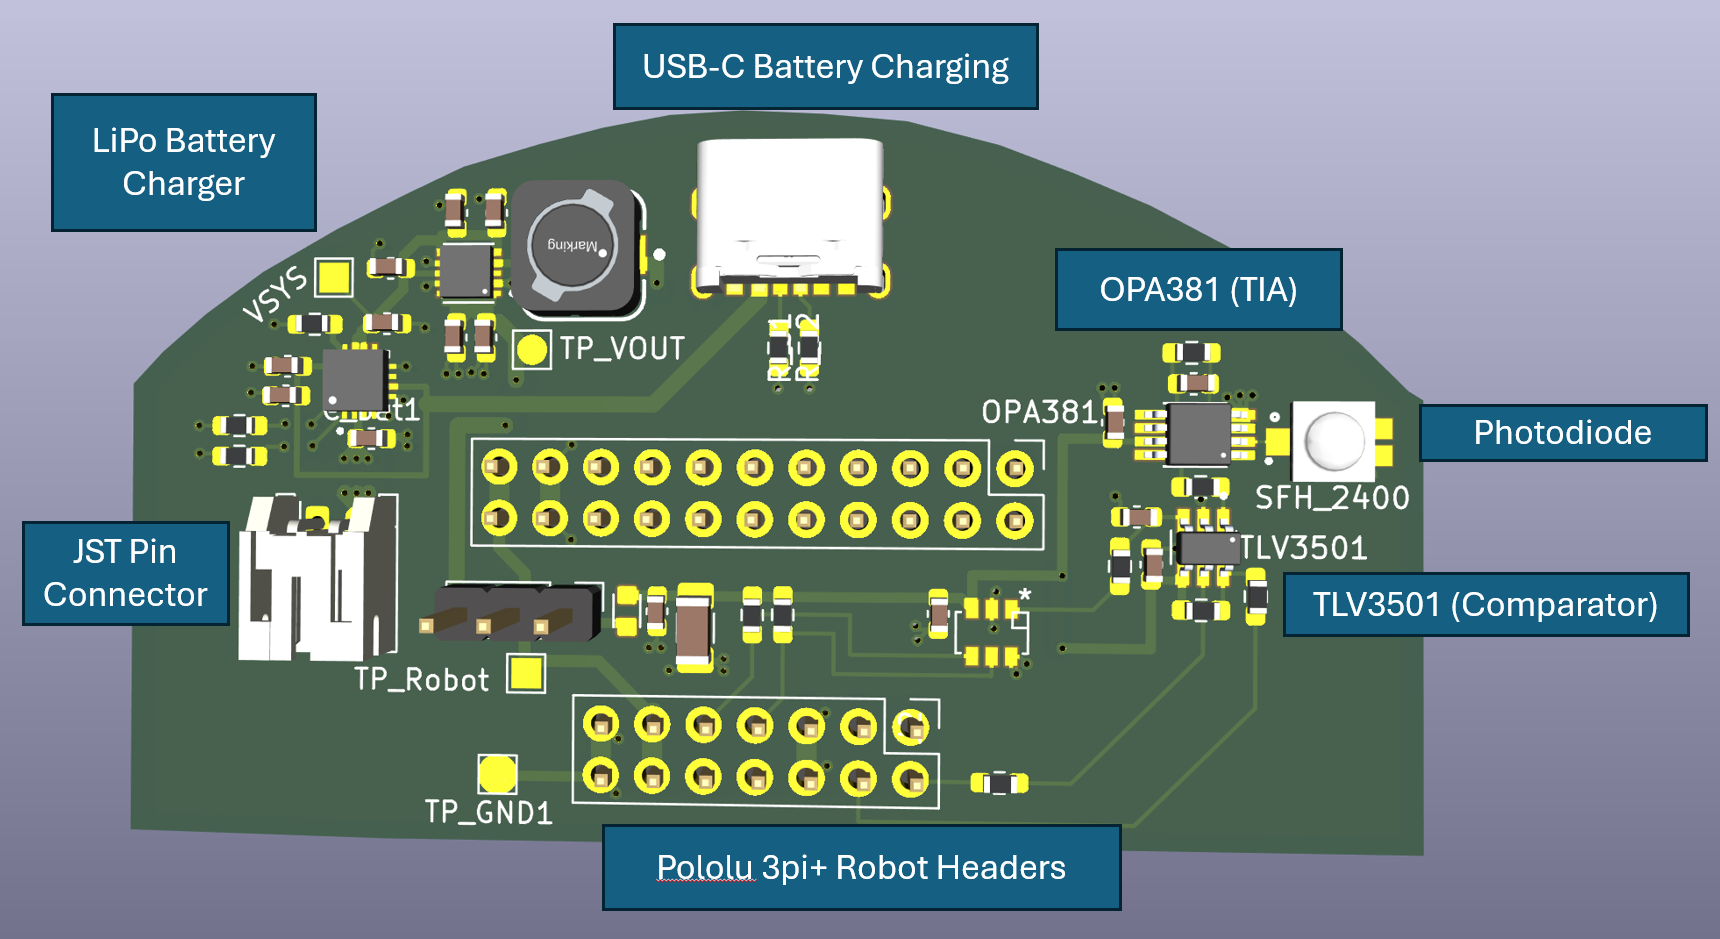
\includegraphics[width=\columnwidth]{lifi_receiver_pcb.png}
\caption{(a) Receiver analog front-end PCB: OPA381AIDGKT TIA, SFH\,2400-Z photodiode, TLV3501AIDBVR comparator, MCP4725 DAC, TPS63031 3.3\,V regulator, BQ24074 LiPo charger, Pololu 3pi+ robot headers, and USB-C charging port.}
\label{fig:receiver_pcb}
\end{figure}

\begin{figure}[h]
\centering
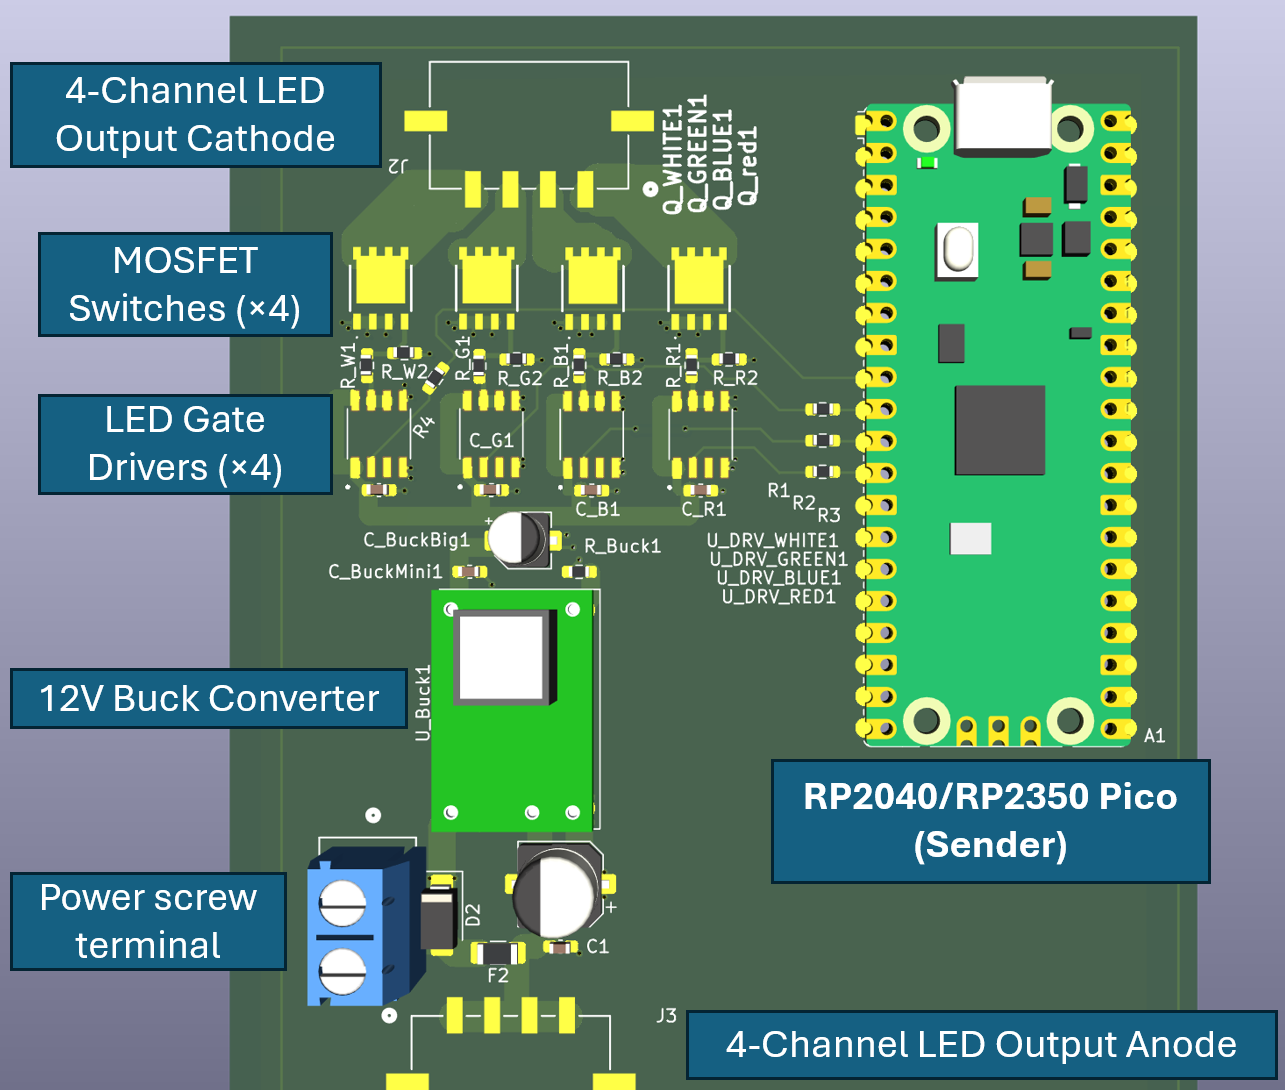
\includegraphics[width=\columnwidth]{lifi_sender_pcb.png}
\caption{(b) Sender LED driver PCB: RP2040/RP2350 Pico, TC4420COA gate drivers ($\times$4), SIR800DP-T1-GE3 MOSFETs ($\times$4), PTN78000WAH 12\,V$\to$5\,V module, and 4-channel LED terminal blocks.}
\label{fig:sender_pcb}
\end{figure}

\subsection{Communication Performance}

Bit-error-rate testing was conducted at a separation distance of approximately 15\,cm between the sender LED array and the receiver photodiode, using the white LED channel with a 50-packet sample per baud rate. Testing was performed under indoor ambient lighting without shielding. The PIO state machine on the RP2040 was configured for 1\,Mbps (clock divider 15.625 at 125\,MHz system clock), and baud rate was swept by adjusting the clock divider.

With $R_f = 470\,\text{k}\Omega$ (2.0\,V output swing), the system achieved 100\% frame success at baud rates up to 300\,kbaud, with hard failure onset above 350\,kbaud. With $R_f = 100\,\text{k}\Omega$ (400\,mV output swing), reliable reception was achieved at up to 250\,kbaud, with complete failure above 400\,kbaud. Notably, the higher-gain 470\,k$\Omega$ configuration outperformed the lower-gain 100\,k$\Omega$ configuration at this distance, indicating that SNR margin from the larger output swing was the dominant factor at close range. At longer distances, the bandwidth advantage of the 100\,k$\Omega$ configuration is expected to dominate as photocurrent decreases and the voltage swing falls below the comparator's noise floor. Extended range and multi-distance characterization are planned for future work.

\subsection{Analog Front-End Characterization}

\begin{table}[htbp]
\caption{TIA Feedback Component Tuning}
\begin{center}
\small
\begin{tabular}{|c|c|c|c|c|}
\hline
$R_f$ & $C_f$ & \textbf{BW (kHz)} & \textbf{Max Baud (meas.)} & \textbf{Swing} \\
\hline
470\,k$\Omega$ & 5\,pF & 68 & 300,000 & $\sim$2.0\,V \\
\hline
100\,k$\Omega$ & 5\,pF & 318 & 250,000 & $\sim$400\,mV \\
\hline
100\,k$\Omega$ & 1\,pF & 1,590 & TBD & $\sim$400\,mV \\
\hline
47\,k$\Omega$ & 1\,pF & 3,386 & TBD & $\sim$200\,mV \\
\hline
\end{tabular}
\label{tab:tia_tuning}
\end{center}
\end{table}

The first two rows of Table~\ref{tab:tia_tuning} have been experimentally validated. The 470\,k$\Omega$ / 5\,pF configuration achieved reliable reception at up to 300\,kbaud at 15\,cm; the 100\,k$\Omega$ / 5\,pF configuration achieved up to 250\,kbaud at the same distance. The lower-resistance configurations (100\,k$\Omega$ / 1\,pF and 47\,k$\Omega$ / 1\,pF) are planned for evaluation in future work targeting data rates above 1\,Mbps.

\subsection{Security Validation}

Authentication is enforced per-frame by the mbedTLS AES-128-GCM implementation. Each received frame is passed to \texttt{mbedtls\_gcm\_auth\_decrypt()}, which verifies the 16-byte GCM authentication tag before returning plaintext. Any frame with a corrupted, truncated, or forged tag causes mbedTLS to return \texttt{MBEDTLS\_ERR\_GCM\_AUTH\_FAILED}; the frame is discarded and the authorization timestamp is not updated. No partial plaintext is released to the application layer prior to successful tag verification — a property guaranteed by the GCM-authenticated decryption interface.

Replay protection is enforced by the 64-entry nonce sliding window. Each incoming frame's 12-byte nonce is checked against the window before decryption is attempted. A frame bearing any nonce already present in the window is rejected without invoking the GCM primitive. Nonce uniqueness within a boot session is guaranteed by the monotonically increasing 32-bit counter field; uniqueness across reboots is ensured with overwhelming probability by the 8-byte random boot salt generated from the RP2040 hardware ring-oscillator entropy source via CTR\_DRBG at startup. Counter exhaustion ($2^{32}$ messages) triggers a device reboot to regenerate the salt, preventing nonce reuse.

Quantitative measurements of tag verification latency and tampered-frame rejection rates across a larger packet sample are planned for a subsequent evaluation campaign.

\subsection{Presence Enforcement}

Authorization revocation upon optical interruption follows directly from the freshness mechanism defined in Section~\ref{eq:freshness}. When the optical path is broken, no new authenticated frames reach the receiver, and the authorization timestamp $t_{\text{last}}$ becomes stale. Within at most $\Delta$ time units, the freshness condition evaluates to false and the receiver revokes authorization without any explicit network-level revocation message.

The configurable token validity window $\Delta$ governs the worst-case revocation latency. For the prototype evaluation, $\Delta$ values in the range of 500\,ms to 2\,s were used, providing a balance between prompt revocation and robustness against momentary optical interruptions (e.g., a person briefly crossing the beam). At a reliable frame rate of 300\,kbaud with standard message sizes, the sender delivers multiple authenticated frames per $\Delta$ interval, ensuring a legitimately positioned receiver maintains continuous authorization without gaps.

Quantitative measurements of worst-case revocation latency and relay attack simulations with measured relay-induced delay are planned for future evaluation.

\section{Discussion}

\subsection{The Bandwidth-Range Tradeoff}

The analog front-end characterization reveals a fundamental tradeoff between communication bandwidth and operational range. The TIA feedback resistor $R_f$ simultaneously controls the gain (and therefore the signal swing available to the comparator) and the bandwidth (and therefore the maximum achievable data rate). Measured results show that at close range (15\,cm), reducing $R_f$ from 470\,k$\Omega$ to 100\,k$\Omega$ did not improve maximum reliable baud rate — the higher-gain 470\,k$\Omega$ configuration achieved 300\,kbaud versus 250\,kbaud for the 100\,k$\Omega$ configuration. This result indicates that at close range, the SNR margin from the larger output swing (2.0\,V vs.\ 400\,mV) is the dominant factor, offsetting the bandwidth advantage of the lower-resistance configuration. At longer operational distances, the balance is expected to shift: as photocurrent decreases, the 2.0\,V swing of the 470\,k$\Omega$ configuration will degrade first, and the higher bandwidth of the 100\,k$\Omega$ configuration will dominate. This reduced swing directly limits the maximum distance at which the comparator can reliably distinguish signal from noise, particularly under ambient light interference.

This tradeoff is not unique to our system --- it is inherent to any transimpedance-based optical receiver --- but it has specific implications for presence-based authorization. A system deployed in a large room with ceiling-mounted LEDs would require higher TIA gain (and therefore lower bandwidth) than a system deployed at close range on a desktop. The programmable DAC threshold partially mitigates this by allowing the comparator decision point to track the reduced swing, but the fundamental sensitivity limit imposed by the photodiode's noise floor and the comparator's 6\,mV hysteresis remains.

Future implementations could address this tradeoff through a dedicated high-bandwidth transimpedance amplifier IC (replacing the general-purpose operational amplifier), a second-stage voltage amplifier to recover signal amplitude after a low-gain TIA, or optical concentrators (lenses, compound parabolic concentrators) on the receiver to increase the effective collection area without modifying the electronics.

\subsection{Relay Attack Resilience}

The $\Delta$-bounded freshness mechanism provides a configurable upper limit on the duration of any relay attack. However, $\Delta$ itself represents a tradeoff: smaller values of $\Delta$ provide tighter relay bounds but require higher frame transmission rates and are more sensitive to momentary optical interruptions (e.g., a person briefly walking through the beam). In practice, $\Delta$ values on the order of 500\,ms to 2\,s appear to provide a reasonable balance between security and robustness for indoor deployments.

A more aggressive relay defense could incorporate challenge-response timing: the receiver periodically challenges the sender with a random nonce, and the sender must respond within a bounded round-trip time. Since the optical channel operates at the speed of light (negligible propagation delay at room scale), any relay that introduces even microseconds of additional latency would be detectable. This extension is architecturally compatible with the existing bidirectional UART link between the sender and receiver but is not implemented in the current prototype.

\subsection{Comparison with RF-Based Alternatives}

The total hardware cost of the prototype is approximately \$82 USD based on verified DigiKey unit pricing (Table~\ref{tab:bom}). The single largest cost driver is the Texas Instruments PTN78000WAH DC-DC power module at \$24.58, selected for its wide input range and module-level integration convenience in the research prototype; a production design substituting a discrete buck regulator IC would reduce system cost to under \$60. By comparison, commercial LiFi systems (e.g., Signify Trulifi) are priced at several thousand dollars per access point, and RF-based physical layer security approaches require specialized antenna arrays, signal processing hardware, and environmental calibration. The open-source nature of both the firmware and the IoTAuth provisioning framework enables reproduction and extension by other researchers without licensing constraints.

More fundamentally, the system provides a security property --- automatic revocation upon physical departure from the optical zone --- that is structurally impossible to achieve with RF-based protocols without environmental modification. No amount of cryptographic sophistication in a WiFi-based system can prevent a device that has authenticated from retaining its credentials after leaving the room, because the RF signal itself does not respect room boundaries. The optical system achieves this property by construction, without any software-level revocation infrastructure.

\subsection{Limitations}

Several limitations of the current implementation should be acknowledged:

\begin{enumerate}
\item \textbf{Line-of-sight requirement.} The system requires an unobstructed optical path between sender and receiver. Environments with significant dust, fog, or vibration may experience intermittent frame loss, triggering unnecessary revocation if $\Delta$ is set too aggressively.

\item \textbf{Single-channel reception.} Although the sender transmits on four LED channels simultaneously, the current receiver uses a single photodiode. Exploiting the spatial diversity of multiple receiver elements could improve robustness and enable angle-of-arrival estimation.

\item \textbf{Ambient light sensitivity.} Strong ambient light sources (direct sunlight, high-intensity discharge lamps) can saturate the photodiode or shift the operating point of the TIA, degrading reception quality. The programmable DAC threshold provides partial mitigation, but a fully adaptive threshold that tracks ambient conditions in real time is not yet implemented.

\item \textbf{No hardware key protection.} The RP2040 and RP2350 do not include a hardware security module or trusted execution environment. Session keys stored in flash are extractable by an adversary with physical access and a debugger. Integration with a Trusted Platform Module (TPM) or secure element would address this limitation.
\end{enumerate}

\section{Future Work}

Several extensions are planned or under consideration:

\begin{enumerate}
\item \textbf{Time-bounded key validity enforcement.} The IoTAuth session key structure includes absolute and relative validity fields (\texttt{abs\_validity}, \texttt{rel\_validity}) that are not yet enforced in firmware. Implementing these timers would enable automatic key expiration and re-provisioning, further limiting the window of exposure if a key is compromised.

\item \textbf{Formal protocol verification.} The security goals G1--G4 are amenable to formal verification using symbolic model checkers such as ProVerif or Tamarin Prover. Modeling the optical channel as a location-restricted link and verifying that the protocol satisfies freshness, replay resistance, and relay-boundedness under the stated adversary model would strengthen the theoretical foundations of this work.

\item \textbf{Multi-sender and multi-receiver environments.} Extending the system to support multiple overlapping optical zones, each with independent session keys and sender identifiers, would enable deployment in open-plan offices, warehouses, and multi-room facilities. The key identifier field in the existing flash block structure provides an architectural anchor for this extension.

\item \textbf{Adaptive threshold control.} Implementing a closed-loop control system that continuously adjusts the MCP4725 DAC threshold based on measured ambient light levels and signal amplitude would improve robustness across varying lighting conditions without manual calibration.

\item \textbf{Higher data rates.} Reducing the TIA feedback resistance to 47\,k$\Omega$ or below with a matched feedback capacitor of 0.5--1\,pF is expected to enable data rates of 2--4\,Mbps. Beyond this, a dedicated high-bandwidth TIA IC and a second-stage amplifier would be required to approach the TLV3501's 80\,MHz toggle limit.

\item \textbf{Optical concentration and collection improvements.} The current prototype operates without any optical shaping on either the transmitter or receiver side. Future iterations will evaluate snap-in collimating lenses (e.g., Carclo 10413, 20--35$^\circ$ beam) on the LED array to narrow and direct the emission cone, improving range and reducing ambient light interference. On the receiver side, a compound parabolic concentrator (CPC) or Fresnel lens positioned over the SFH\,2400-Z photodiode can increase the effective optical collection area by an order of magnitude, extending operational range without modifying the electronic signal chain. Reflective funnel structures mounted directly on the photodiode aperture are also under consideration to improve signal capture in diffuse or off-axis illumination conditions.

\item \textbf{Hardware key protection.} Integrating a TPM or secure element (e.g., ATECC608) for session key storage would prevent key extraction via physical access, addressing the most significant limitation of the current microcontroller-only implementation.

\item \textbf{Robotic platform demonstration.} The receiver PCB is already designed with Pololu 3pi+ robot integration headers and an onboard LiPo power system. Deploying the complete receiver on a 3pi+ platform and demonstrating that the robot executes commands only while continuously receiving authenticated optical frames --- and halts immediately upon optical interruption --- would provide a compelling physical demonstration of presence-based authorization in a mobile cyber-physical system context.
\end{enumerate}

\section{Conclusion}

This work presents the design, implementation, and initial evaluation of a presence-based authorization system that uses LiFi optical communication as both a data channel and a physical security primitive. Unlike conventional authentication models --- in which a device that has verified its identity retains access until explicitly revoked --- the proposed system continuously binds authorization to the physical reception of authenticated optical frames, such that access is automatically revoked within a configurable time window $\Delta$ upon interruption of the optical path.

The system achieves authenticated encryption at 1\,Mbps over a free-space optical link using AES-128-GCM on commodity microcontrollers (RP2040 and RP2350), with a custom analog front-end comprising an OPA381AIDGKT precision transimpedance amplifier, TLV3501AIDBVR high-speed comparator, and MCP4725A1T-E/CH programmable DAC threshold. Session keys are provisioned through the IoTAuth framework with HMAC-SHA256 challenge-response authentication and persisted in a dual-slot flash architecture with SHA-256 integrity verification. A 64-entry nonce sliding window provides replay attack prevention, and the token validity window $\Delta$ bounds the advantage of relay attacks.

The total hardware cost of the prototype is approximately \$82 USD at verified DigiKey unit pricing, demonstrating that presence-based optical authorization is achievable on resource-constrained embedded platforms without specialized or expensive hardware --- remaining two orders of magnitude below commercial LiFi access point pricing. The analog front-end characterization reveals a quantifiable tradeoff between TIA bandwidth and operational range --- a result that directly informs the design of future deployments.

By formalizing the security goals of freshness, replay resistance, relay-bounded authorization, and revocation on interruption, and by demonstrating their enforcement through a physical prototype, this work establishes that light itself --- confined by physics, modulated by electronics, and authenticated by cryptography --- can serve as a verifiable and continuously enforced proof of physical presence.

\section*{Acknowledgment}

The authors thank KIM Labs at Arizona State University for providing the facilities and resources used in this work.

\begin{thebibliography}{00}

\bibitem{wyner1975}
A. D. Wyner, ``The Wire-Tap Channel,'' \textit{Bell System Technical Journal}, vol. 54, no. 8, pp. 1355--1387, Oct. 1975.

\bibitem{brands1993}
S. Brands and D. Chaum, ``Distance-Bounding Protocols,'' in \textit{Advances in Cryptology --- EUROCRYPT '93}, Lecture Notes in Computer Science, vol. 765, Springer, Berlin, 1994, pp. 344--359.

\bibitem{haas2011}
H. Haas, ``Wireless data from every light bulb,'' TEDGlobal, Edinburgh, July 2011.

\bibitem{ieee80211bb}
IEEE, ``IEEE Standard for Information Technology --- Local and Metropolitan Area Networks --- Specific Requirements --- Part 11: Wireless LAN Medium Access Control (MAC) and Physical Layer (PHY) Specifications Amendment 7: Light Communications,'' \textit{IEEE Std 802.11bb-2023}, 2023.

\bibitem{blinowski2019}
G. Blinowski, ``Security of Visible Light Communication systems --- A survey,'' \textit{Physical Communication}, vol. 34, pp. 246--256, June 2019.

\bibitem{arfaoui2020}
M. A. Arfaoui, M. D. Soltani, I. Tavakkolnia, A. Ghrayeb, M. Safari, C. Assi, and H. Haas, ``Physical Layer Security for Visible Light Communication Systems: A Survey,'' \textit{IEEE Communications Surveys \& Tutorials}, vol. 22, no. 3, pp. 1887--1908, 2020.

\bibitem{cho2018}
S. Cho, G. Chen, and J. P. Coon, ``Securing visible light communication systems by beamforming in the presence of randomly distributed eavesdroppers,'' \textit{IEEE Trans. Wireless Commun.}, vol. 17, no. 5, pp. 2918--2931, May 2018.

\bibitem{irs_vlc2024}
M. Caputo, M. Mucchi, and L. Pierucci, ``Multi-RIS Aided VLC Physical Layer Security for 6G Wireless Networks,'' \textit{IEEE Trans. Inf. Forensics Security}, 2024.

\bibitem{almoliki2017}
Y. M. Al-Moliki, M. T. Alresheedi, and Y. Al-Harthi, ``A Physical Layer Security Key Generation Technique for Inter-Vehicular Visible Light Communication,'' in \textit{Proc. IEEE Int. Conf. Commun.}, 2017.

\bibitem{keygen_ofdm2017}
R. Marin-Garcia, R. Perez-Jimenez, and B. Alonso-Gonzalez, ``Secret Key Generation Protocol for Optical OFDM Systems in Indoor VLC Networks,'' \textit{IEEE Photonics Technology Letters}, 2017.

\bibitem{qkd_vlc2025}
M. S. Hossain et al., ``Secure Quantum Key Distribution Over VLC Networks for Next-Generation Smart Cities,'' \textit{Int. J. Networked Distrib. Comput.}, 2025.

\bibitem{lisa2019}
N. Saxena, J. Y. Choi, and S. Cho, ``LISA: Visible light based initialization and SMS based authentication of constrained IoT devices,'' \textit{Future Generation Computer Systems}, vol. 93, pp. 167--178, Apr. 2019.

\bibitem{kim2020}
S.-M. Kim, ``Secure Visible Light Communication Technique Based on Asymmetric Data Encryption for 6G Communication Service,'' \textit{Electronics}, vol. 9, no. 11, p. 1847, Nov. 2020.

\bibitem{liao2021}
T.-L. Liao, C.-Y. Chen, H.-C. Chen, Y.-Y. Chen, and Y.-Y. Hou, ``Realization of a Secure Visible Light Communication System via Chaos Synchronization,'' \textit{Mathematical Problems in Engineering}, vol. 2021, Feb. 2021.

\bibitem{signify2024}
Signify N.V., ``Trulifi: High-speed Internet using your lights with LiFi,'' 2024. [Online]. Available: \url{https://www.signify.com/global/innovation/trulifi}

\bibitem{oledcomm2024}
Oledcomm S.A.S., ``LiFi Technology for Cybersecurity Solutions,'' 2024. [Online]. Available: \url{https://www.oledcomm.net/solutions/cybersecurity/}

\bibitem{lifilab2024}
LiFi Lab, ``LiFi Secure Access Control System,'' 2024. [Online]. Available: \url{https://lifi-lab.com/tecnologia-lifi/lifi-secure-access-eng/}

\end{thebibliography}

\end{document}
